\documentclass{beamer}
\mode<presentation> {
\usetheme{CambridgeUS}
}
%\usecolortheme[named=blue]{structure}
\usepackage{xcolor}
\usepackage{graphicx} % Allows including images
%	TITLE PAGE
\title[Department of Mathematics]{Pricing European barrier options with rebates}
\institute[] 
{\textbf{Department of Mathematics\\
International University} \\
\medskip
	\begin{figure}[htp]
	\begin{center}
		
\includegraphics[scale=.2]{logo}
	\end{center}
	\label{reflogo}
\end{figure}

\text{Author: Ta Thi Phuong Dung} \\
\text{Advisor: Dr. Le Nhat Tan} 
}
\date{\today}

\begin{document}

\begin{frame}
\titlepage 
\end{frame}
\begin{frame}
\frametitle{Outline} 
\tableofcontents
\end{frame}

\section{Introdution}
\begin{frame}
\begin{figure}[htp]
	\begin{center}
		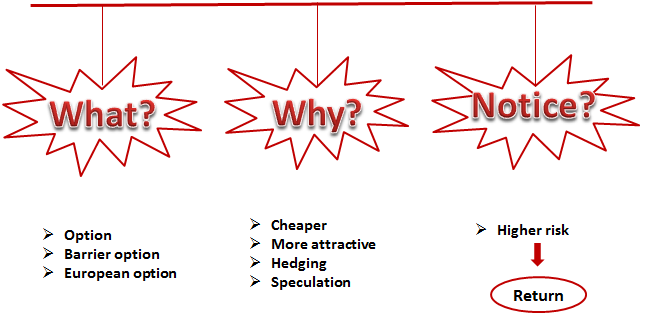
\includegraphics[scale=0.5]{fig7}
	\end{center}
\end{figure} \pause
\begin{itemize}
	\item On August 10, 2017, the VN30-Index futures contract were officially traded in the Vietnam market
	\item Next April, Coverall call option is expected to open. \\[0.3cm]
	\item Pricing options is very urgent\\[0.3cm]
	$\Rightarrow$ Using the probabilistic approach for formulating the pricing models
\end{itemize}
\end{frame}

\begin{frame}
\frametitle{European barrier options with rebates}
\begin{figure}[htp]
	\begin{center}
		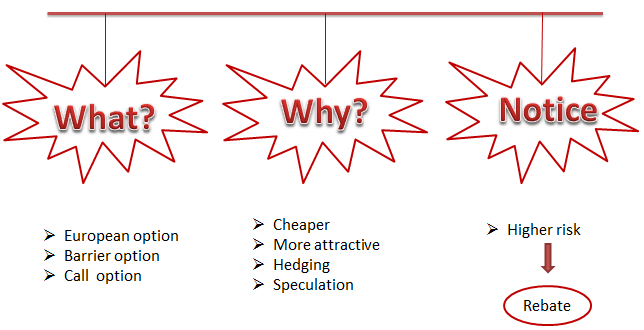
\includegraphics[scale=0.6]{fig8}
	\end{center}
\end{figure}
\end{frame}

%------------------------------------------------
\section{Pricing European barrier call options with rebates}
\begin{frame}
\frametitle{Option price}
\begin{figure}[htp]
	\begin{center}
		
\includegraphics[scale=0.6]{fig9}
	\end{center} \pause 
\begin{center}
	
\includegraphics[scale=0.6]{fig10}
\end{center}
\end{figure}	
\end{frame}
\begin{frame}
\frametitle{Pricing option procedure}
Option price at expiry is known from definition
\begin{align}
	C_{d/o}(S_T)=\max\{S_T-K, 0\}\mathcal{H}_{\{min_{t\leq u\leq T}S_u > B\}}
\end{align}
The stock price $S_t$ follows a geometric Brownian motion with the following SDE
\begin{align*}
\dfrac{dS_t}{S_t}=\mu dt+\sigma dW_t
\end{align*}
where $\mu$ is the drift parameter and $\sigma$ is the volatility parameter.\\[0.5cm]
Risk-neutral measure
\begin{align*}
	\dfrac{dS_t}{S_t}=r dt+\sigma dW_t
\end{align*}
\end{frame}
%------------------------------------------------
\begin{frame}
\frametitle{Pricing option procedure}
By solving SDE, 
\begin{align*}
S_t=S_0e^{\left(r -\frac{1}{2}\sigma^2 \right)t+\sigma W_t^{\mathbb{Q}}} \end{align*} 
Let's consider times from $t$ to $T$ for $t<T$, we obtain
\begin{align*}
	S_T&=S_te^{\left(r -\frac{1}{2}\sigma^2 \right)(T-t)+\sigma W_{T-t}^\mathbb{Q}}\\
	&=S_te^{\sigma \widehat{W}_{T-t}}
\end{align*}
where $\widehat{W}_{T-t}=\nu (T-t)+W_{T-t}^\mathbb{Q}$ and $\nu=\dfrac{1}{\sigma}(r-\dfrac{1}{2}\sigma^2)$. By writing
\begin{align*}
m_{T-t}=min_{t\leq u \leq T}\widehat{W}_{u-t}
\end{align*}
Therefore, 
\begin{align*}
\displaystyle \min_{t\leq u \leq T}S_u=S_te^{\sigma 	m_{T-t}}
\end{align*} 
\end{frame}
\begin{frame}
\frametitle{Pricing option procedure}
and we can rewrite the payoff as 
\begin{align*}
C_{d/o}(S_T)&=(S_te^{\sigma \widehat{W}_{T-t}}-K)\mathcal{H}_{\{m_{T-t}>\frac{1}{\sigma}\log\left(\frac{B}{S_t}\right), \widehat{W}_{T-t}>\frac{1}{\sigma}log\left(\frac{K}{S_t}\right) \}} \\
C_{d/o}(S_t)&=e^{-r(T-t)}\displaystyle \int_{\omega =\frac{1}{\sigma}log\left(\frac{K}{S_t}\right) }^{\infty}\displaystyle \int_{m =\frac{1}{\sigma}log\left(\frac{B}{S_t}\right) }^{m=\omega}(S_te^{\sigma \omega}-K)f^\mathbb{Q}_{m,\widehat{W}}(m, \omega)dmd\omega\\
&=C_{bs}(S_t,t;K,T)-\left(\dfrac{S_t}{B}\right)^{2\lambda}C_{bs}(\dfrac{B^2}{S_t},t;K,T)
\end{align*}
where $\lambda = \dfrac{1}{2}\left(1-\dfrac{r}{\frac{1}{2}\sigma^2}\right)$ and \\[0.2cm]
$C_{bs}(S_t,t;K,T)=S_tN(d_1)-Ke^{-r(T-t)}N(d2)$\\[0.2cm]
$d_1=\dfrac{log(S_t/K)+(r+\frac{1}{2}\sigma^2)(T-t)}{\sigma\sqrt{T-t}}, \hspace{0.2cm}d_2=d_1-\sigma\sqrt{T-t}$
\end{frame}
\begin{frame}
\frametitle{Pricing option procedure}
$C_{bs}(\dfrac{B^2}{S_t},t;K,T)=\dfrac{B^2}{S_t}N(d_3)-Ke^{-r(T-t)}N(d4)$\\[0.2cm]
$d_3=\dfrac{log(B^2/(S_tK))+(r+\frac{1}{2}\sigma^2)(T-t)}{\sigma\sqrt{T-t}}, \hspace{0.2cm}d_4=d_3-\sigma\sqrt{T-t}$\\
The expected present value of the rebate is given by \\ [0.2cm]

$\textnormal{Rebates value}=R \displaystyle \int_{0}^{T} e^{-ru}Q(u; B)du$\\ [0.2cm]
$=R\left[\left(\dfrac{B}{S}\right)^{\alpha_+}\Phi\left(-\dfrac{\ln \frac{B}{S}+\beta T}{\sigma\sqrt{T}}\right)+\left(\dfrac{B}{S}\right)^{\alpha_-}\Phi\left(-\dfrac{\ln \frac{B}{S}-\beta T}{\sigma\sqrt{T}}\right)\right]$\\ [0.2cm]
where
\begin{align*}
\beta=\sqrt{\left(r-\dfrac{\sigma^2}{2}\right)^2+2r\sigma^2}, \hspace{0.2cm} \alpha_\pm = \dfrac{r-\frac{\sigma^2}{2}\pm B}{\sigma^2}
\end{align*}	
\end{frame}
\begin{frame}
	\frametitle{Pricing option procedure}
	\begin{block}{{\color{red} \bfseries {The final result}}}
	\begin{align*}
		C^R_{d/o}(S_t,t;K,B,T)=C_{bs}(S_t,t;K,T)-\left(\dfrac{S_t}{B}\right)^{2\lambda}C_{bs}(\dfrac{B^2}{S_t},t;K,T)\\
		+R\left[\left(\dfrac{B}{S}\right)^{\alpha_+}\Phi\left(-\dfrac{\ln \frac{B}{S}+\beta T}{\sigma\sqrt{T}}\right)+\left(\dfrac{B}{S}\right)^{\alpha_-}\Phi\left(-\dfrac{\ln \frac{B}{S}-\beta T}{\sigma\sqrt{T}}\right)\right]
	\end{align*}
	\end{block}
\end{frame}
\section{Application}
\begin{frame}
\frametitle{Under Black-Scholes model's assumption}
Pricing European barrier call option with reabtes on FPT stock.\\
Source: \url{http://www.cophieu68.vn/historyprice.php?id=fpt}\\
Daily return $u_i=\ln\dfrac{S_i}{S_{i-1}} \hspace{0.4cm} \text{for}\hspace{0.2cm}i=0, 1, \dots, n$ \\ \pause
\fontsize{9pt}{10pt}\selectfont {\color{red} Testing for normal distribution}\\[0.2cm]
Using graphical methods: Q-Q plot. Our result
\begin{figure}[htp]
	\begin{center}
		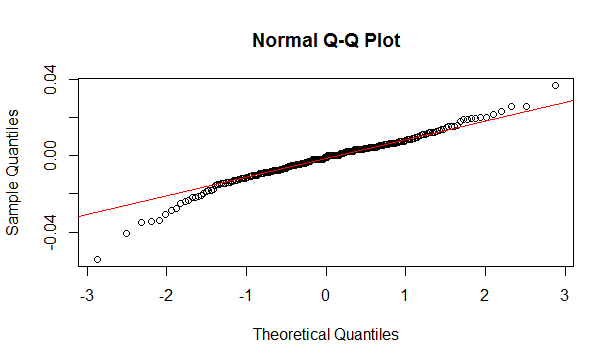
\includegraphics[scale=.4]{Rplot03}
	\end{center}
	\label{refRplot03}
	\caption{The distribution of FPT stock}
\end{figure}
\end{frame}
\begin{frame}
 \frametitle{Applied}
 Parameters is given by
 \begin{table}[!htp]
 	\centering
 	\begin{tabular}{|l|c|r|}
 		\hline
 		$S_0$ & Stock price at time zero   & $59.8$ VND\\
 		\hline
 		$K$ & Strike price  & $62$ VND\\
 		\hline
 		$\sigma$ &  Annual volitility & $24\%$\\
 		\hline
 		$r$ & Annual riskless rate  & $3\%$ \\
 		\hline
 		$T$ & Option expiration (in years)  & $0.5$\\
 		\hline	
 	\end{tabular}
 	\caption{FPT stock}
 \end{table} \pause
Substitute the above data into the final result, we obtain
\begin{align*}
C^R_{d/o}(S_t,t;K,B,T)=9.02944 
\end{align*}
This means that a European barrier down-and-out call option with rebates under FPT stock has price of $9.03$ VND.
\end{frame}
\section{Conclusion}
\begin{frame}

{\color{red} \bfseries {Conclusion}}
\begin{itemize}
	\item Mathematical techniques: Probabilistic approach\\[0.2cm]
	\item Be essential to Vietnam market, especially Derivatives 
\end{itemize} 

\vspace{0.5cm}
{\color{red} \bfseries {Limitations}}
\begin{itemize}
	\item Following Black-Scholes model's assupmtion
\end{itemize}
\end{frame}
\begin{frame}
	\begin{figure}[htp]
		\begin{center}
			
\includegraphics[scale=0.8]{fig11}
		\end{center}
	\end{figure}
\end{frame}
\end{document} 